
\subsection{Requirements (Aims)}

Our aim is to create a distributed chat system with the following specific requirements by  priority.

\begin{table}[ht]
\caption{Requirements by priority level}
\label{tab:requirements}
    \begin{tabular}[c]{ | p{5cm} | p{5cm} | p{5cm} |}
		\hline
		\centering\textbf{Priority 1} & \centering{\textbf{Priority 2}} & \centering\textbf{Priority 3} &
    \hline
    \parbox[t]{5cm}{-Secure connection\\-Encrypted messages\\ -iOS, Android and Web platforms (at least two platforms)\\ -Contact list\\ -Search for contacts\\ -Sign in by email or Gmail \\ -One to one conversation (text message)} &  \parbox[t]{5cm}{-Send images\\ -Group chat\\ -Chat bubbles instead of username\\ -Notifications of received messages}
& \parbox[t]{5cm}{-Sign Up with Facebook\\ -Availability to send other type of media (e.g. video, voice notes, etc.)\\ -Online status of other users\\ -Acknowledgment of received, delivered and read messages, including date time\\ -Ability to use the chat offline}\\
    \hline
    \end{tabular}
\end{table}


\subsection{Strategy and Timetable}

Our strategy is to develop three client-based platforms (i.e. Android, iOS and Web) using Firebase as a server. The reason for including a third platform is to act as a backup should there be problem with any of the platforms during testing which we are unable to debug at the end. The tentative timetable (Figure ~\ref{fig:timetable}) presents the main activities required to complete our final product. It is important to state that the timetable and our strategy is constructed based on the Scrum ~\cite{scrum} methodology, which  is an agile software development guide that allows us to iterate and make incremental and evolutionary contributions.  We will also use different Project Management roles like a Scrum Master (who removes team obstacles and pushes resolutions) and the product owner (who acts as the client voice) to ensure a high-quality product. The main activities are explained as follows: 

\begin{enumerate}
	\item \textbf{Plan}: Here we defined how we are going to work, our goals and organization as a team. We also discussed our individual strengths and weaknesses and the tools available to achieve our aim and objectives.
	\item \textbf{Firebase}: For simplicity, costs (free) and security we are using this Backend as a Service platform to have a robust system which takes care of the authentication, rules for accessing the database (read/write) and the storage of documents so that we could focus on the core functionality, i.e. the actual messaging.
	\item \textbf{UI}: Refers to designing the User Interfaces for all the clients.
	\item \textbf{Client Development}: This is the development of the specific application for each type of client (Android, iOS and Web): 
	\begin{enumerate}
		\item \textbf{Setup}: Here we add the required files and initialize the repository on GitHub. Then we create the project on Firebase so that we could share the same API Keys.
		\item \textbf{Login}: Build the login page, authentication using email and password, Gmail and Facebook if possible.
		\item \textbf{Conversations}: Text messaging between clients using Firebase as a central database containing the messages between recipients and taking care of the encryption. Add chat bubbles, send and receive messages, show them in an organized manner with timestamps.  
		\item \textbf{Image Message}: Share images inside messages (nice to have).
	\end{enumerate}
		\item \textbf{Integration Testing}: Test functionality across platforms. 
		\item \textbf{Quality Assurance}: Check that all clients communicate with the backend as intended in order to ensure that we cover all the required functionalities and fix any problem that we may have.	
\end{enumerate}

\begin{figure}[ht]
%[Parzen Window Estimated Distributions]
\centering
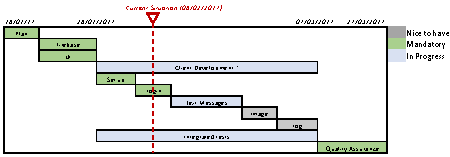
\includegraphics[width=0.9\textwidth]{figs/Timetable}
	\caption{Timetable}
	\label{fig:timetable}
\end{figure}


Please note that our activities in the client development are organized by hierarchy over time. Thus, developing the text message functionality (which is mandatory) is more important than the image message functionality (which is optional but highly desirable). Consequently, we decomposed our activities into tasks and allocated them to each team member as follows:

\begin{figure}[ht]
%[Parzen Window Estimated Distributions]
\centering
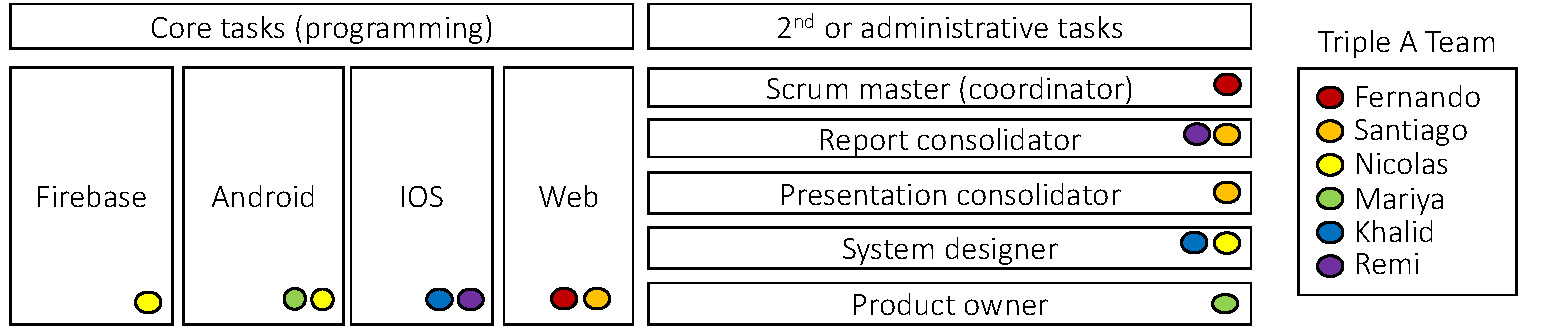
\includegraphics[width=1\textwidth]{figs/tasks}
	\caption{Tasks allocation}
	\label{fig:Tasks}
\end{figure}

\subsection{Current State}
Currently, we have developed the authentication functionality inside the three clients. Firebase authorizes the logged users and allows them see the data only if they are logged in.

\subsection{Next Steps}
Following our timetable, we are going to focus on making the proper database structure (chats, messages, users, receiver, sender, type of message, etc), rules for accessing the data inside the database (only user x and user y can see their own conversation) and adding new data to the database.